
\begin{tblr}{|Q[c,m]|l|l|}
	\hline
	\SetCell[c=3]{c} Maria \\
	\hline
	Tentativas & Medição & Desvio Padrão \\ \hline
	1 &   &  \\\hline
	2 &   &  \\\hline
	3 &   &  \\\hline
	4 &   &  \\\hline
	5 &   &  \\\hline
	6 &   &  \\\hline
	7 &   &  \\\hline
	8 &   &  \\\hline
	9 &   &  \\\hline
	10 &  &  \\\hline
	11 &  &  \\\hline
	12 &  &  \\\hline
	13 &  &  \\\hline
	14 &  &  \\\hline
	15 &  &  \\\hline
	16 &  &  \\\hline
	17 &  &  \\\hline
	18 &  &  \\\hline
	19 &  &  \\\hline
	20 &  &  \\\hline
	\hline
	Média & & $\pm$ \\ \hline
	\hline
\end{tblr}

\begin{tblr}{|Q[c,m]|l|l|}
	\hline
	\SetCell[c=3]{c} Paulina \\
	\hline
	Tentativas & Medição & Desvio Padrão \\ \hline
	1 &   &  \\\hline
	2 &   &  \\\hline
	3 &   &  \\\hline
	4 &   &  \\\hline
	5 &   &  \\\hline
	6 &   &  \\\hline
	7 &   &  \\\hline
	8 &   &  \\\hline
	9 &   &  \\\hline
	10 &  &  \\\hline
	11 &  &  \\\hline
	12 &  &  \\\hline
	13 &  &  \\\hline
	14 &  &  \\\hline
	15 &  &  \\\hline
	16 &  &  \\\hline
	17 &  &  \\\hline
	18 &  &  \\\hline
	19 &  &  \\\hline
	20 &  &  \\\hline
	\hline
	Média & & $\pm$ \\ \hline
	\hline
\end{tblr}

\begin{tblr}{|Q[c,m]|l|l|}
	\hline
	\SetCell[c=3]{c} Marco \\
	\hline
	Tentativas & Medição & Desvio Padrão \\ \hline
	1 &   &  \\\hline
	2 &   &  \\\hline
	3 &   &  \\\hline
	4 &   &  \\\hline
	5 &   &  \\\hline
	6 &   &  \\\hline
	7 &   &  \\\hline
	8 &   &  \\\hline
	9 &   &  \\\hline
	10 &  &  \\\hline
	11 &  &  \\\hline
	12 &  &  \\\hline
	13 &  &  \\\hline
	14 &  &  \\\hline
	15 &  &  \\\hline
	16 &  &  \\\hline
	17 &  &  \\\hline
	18 &  &  \\\hline
	19 &  &  \\\hline
	20 &  &  \\\hline
	\hline
	Média & & $\pm$ \\ \hline
	\hline
\end{tblr}

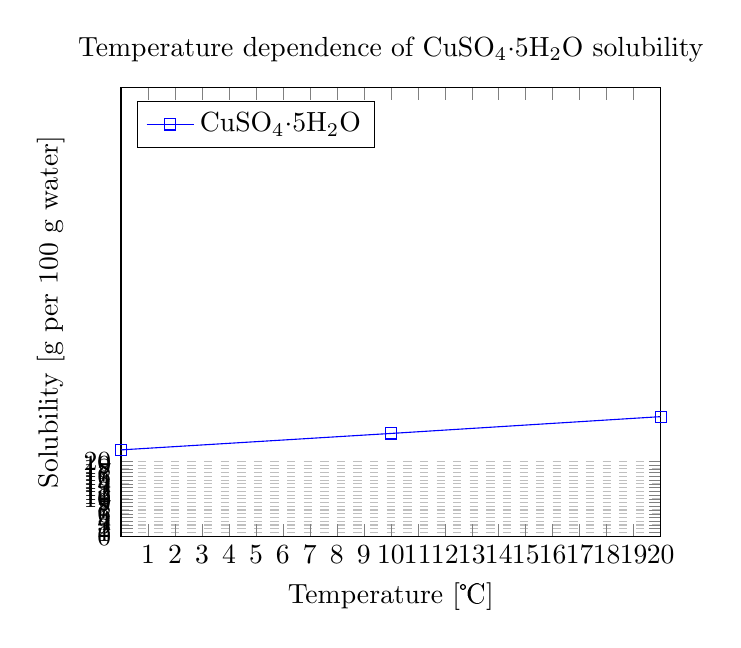
\begin{tikzpicture}
	\begin{axis}[
		title={Temperature dependence of CuSO\(_4\cdot\)5H\(_2\)O solubility},
		xlabel={Temperature [\textcelsius]},
		ylabel={Solubility [g per 100 g water]},
		xmin=0, xmax=20,
		ymin=0, ymax=120,
		xtick={1,2,3,4,5,6,7,8,9,10,11,12,13,14,15,16,17,18,19,20},
		ytick={0,1,2,3,4,5,6,7,8,9,10,11,12,13,14,15,16,17,18,19,20},
		legend pos=north west,
		ymajorgrids=true,
		grid style=dashed,
		]
		
		\addplot[
		color=blue,
		mark=square,
		]
		coordinates {
			(0,23.1)(10,27.5)(20,32)(30,37.8)(40,44.6)(60,61.8)(80,83.8)(100,114)
		};
		\legend{CuSO\(_4\cdot\)5H\(_2\)O}
		
	\end{axis}
\end{tikzpicture}
\vspace{5mm}

